\subsection{Verso la Product Baseline}

\subsubsection{Pianificazione}
Periodo previsto: 16/01/2024-12/03/2024\\ 
\vspace{0.2cm} 
Periodo effettivo: (??)-(??)\\ 
\vspace{0.2cm} 
In questa sezione, pur avendo un'idea di ciò che ci attende, al momento abbiamo scelto di strutturare i nostri periodi di lavoro in fasi più lunghe anziché bisettimanali. Questa decisione deriva dalla nostra attuale valutazione delle competenze, poiché riteniamo prematuro definire l'intervallo che precede la seconda revisione con periodi di tempo molto definiti e stretti.

Le fasi attuali, più lunghe e meno specifiche, saranno progressivamente convertite in periodi bisettimanali quando vi sarà una maggiore consapevolezza delle \textit{attività}\textsubscript{\textit{G}} future.

\vspace{0.2cm}

\textbf{Obiettivo}: Nella fase successiva, il focus sarà sullo sviluppo dei Diagrammi delle Classi e di eventuali nuovi documenti. L'obiettivo primario sarà la realizzazione del prodotto effettivo partendo dal \textit{POC}\textsubscript{\textit{G}}, integrando le funzionalità non ancora implementate e migliorandolo nei punti più deboli della sua struttura.

\todo{da rivedere questa parte introduttiva}

\paragraph{Prima fase}
Intervallo temporale previsto: 16/01/2024-13/02/2024\\ 
\vspace{0.2cm} 
Durante la prima fase, l'attenzione sarà rivolta all'inizializzazione di possibili nuovi documenti per la \textit{PB}\textsubscript{\textit{G}}, in parallelo sarà affrontato lo studio dell'\textit{architettura}\textsubscript{\textit{G}} di \textit{sistema}\textsubscript{\textit{G}} e dei design \textit{pattern}\textsubscript{\textit{G}} più appropriati.

\vspace{0.2cm}

I lavori continueranno sul \textit{Piano di Progetto}, sulla correzione dei documenti \textit{Analisi dei Requisiti}, \textit{Glossario} e \textit{Piano di Qualifica}. Si avvierà la realizzazione dei diagrammi di \textit{attività}\textsubscript{\textit{G}} e sequenze, dando anche inizio allo sviluppo della prima versione del prodotto basata sul \textit{PoC}\textsubscript{\textit{G}}.

\paragraph{Seconda fase}
Intervallo temporale previsto: 13/02/2024-12/03/2024
\\ 
\vspace{0.2cm} 
Durante la seconda fase del progetto, l'attenzione sarà rivolta all’avanzamento di possibili nuovi documenti per la \textit{PB}\textsubscript{\textit{G}}, insieme alla continuazione dei documenti inizialmente avviati. In parallelo, saranno eseguite ottimizzazioni del \textit{sistema}\textsubscript{\textit{G}}, attraverso \textit{test}\textsubscript{\textit{G}} specifici per valutare la sua scalabilità e l'implementazione di allarmi per individuare eventuali anomalie o superamento di soglie critiche.

Si proseguirà con il perfezionamento del codice stesso, garantendo un costante miglioramento delle funzionalità e delle prestazioni del prodotto in fase di sviluppo.

\paragraph{Terza fase}
Intervallo temporale previsto: 12/03/2024-25/03/2024\\ 
\vspace{0.2cm} 
Durante la terza fase del nostro progetto, l'attenzione sarà rivolta all'ultimazione delle nuove versioni del \textit{Piano di Qualifica}, delle \textit{Norme di Progetto}, del \textit{Glossario} e del \textit{Piano di Qualifica}, completando contemporaneamente i documenti specifici della revisione \textit{PB}\textsubscript{\textit{G}}.

Sarà inoltre intensivamente testato il prodotto attraverso i \textit{test}\textsubscript{\textit{G}} e le metriche descritte all'interno del documento \textit{Piano di Qualifica} ed infine verrà creata la presentazione per la \textit{PB}\textsubscript{\textit{G}}.


%---------------------OTTAVO PERIODO---------------------------------------

\subsubsection{Ottavo periodo  16/02/2024 - 23/02/2024}
\paragraph{Considerazioni}

Gli obiettivi principali programmati per l’ottavo periodo riguardano l’esecuzione della seconda fase della revisione RTB e l’inizio delle prime attività in vista della revisione PB. \\
Durante la prima metà dell’ottavo periodo infatti, il team ha dedicato la propria attenzione alla preparazione della presentazione del prodotto per la seconda fase della revisione RTB. Dopo aver apportato alcune lievi modifiche alla documentazione, il focus è stato interamente rivolto alla creazione della presentazione in vista della revisione. Infine, il Responsabile ha effettuato le operazioni necessarie per organizzare e richiedere il colloquio con il Prof. Vardanega. In aggiunta, sono state finalizzate le correzioni segnalate dal Prof. Cardin al documento “\textit{Analisi dei Requisiti}”. \\
Il 20/02/2024 si è svolta la seconda fase della revisione RTB, la quale ha avuto esito positivo e, in seguito alla ricezione della valutazione, sono state avviate le azioni correttive segnalate ai documenti presentati alla revisione. \\
Successivamente, sono state pianificate le prime attività in vista della revisione PB, la quale, ha come obiettivo primario la consegna di un MVP. Di conseguenza, notevoli risorse sono state destinate ai ruoli di Progettisti e Programmatori. \\
Le attività principali del gruppo hanno riguardato la progettazione e lo sviluppo dei simulatori dei sensori, del database per la memorizzazione permanente delle misurazioni e della dashboard per la visualizzazione e l’analisi dei dati.
Contemporaneamente, è iniziata la redazione delle prime sezioni del documento "\textit{Specifica Tecnica}", in cui verranno approfonditi tutti gli aspetti relativi al design del sistema. In particolare, è stata redatta una stesura preliminare della sezione di introduzione e della sezione relativa alle scelte tecnologiche.
Inoltre, tra le attività pianificate, sono in corso analisi mirate a individuare la strategia ottimale per condurre test di integrazione automatizzati al fine di garantire che le misurazioni vengano trasmesse correttamente dai simulatori a Kafka e da Kafka al database Clickhouse. \\
Durante il SAL datato 23/02/2024, come riportato nel relativo \textit{verbale esterno}, la proponente ha richiesto la modifica della configurazione del database in quanto ritenuta sovraingegnerizzata e difficilmente manutenibile. Pertanto, nel nono periodo sarà necessario destinare risorse alla realizzazione di tali modifiche, alla finalizzazione della dashboard e allo sviluppo dei test.

\paragraph{Gestione dei rischi} 

\begin{itemize}
    \item \textbf{Rischi attesi e verificati:}
\begin{itemize}
    \item \textbf{ID} - \textcolor{red}{Inesperienza nell'attività di progettazione} (\textit{inserisci riferimento})
    \item \textbf{ID} - \textcolor{red}{Inesperienza nell'attività di testing} (\textit{inserisci riferimento})
\end{itemize}
\item \textbf{Rischi attesi ma non verificati:} \todo{completa}
 \begin{itemize}
    \item \textbf{RO-2M-2} - Ritardo nel completamento delle \textit{attività}\textsubscript{\textit{G}} rispetto ai tempi previsti~(\ref{sec:ritAttivita});
    \item \textbf{RP-2B-1} - Contrasti interni al gruppo~(\textit{\ref{subsubsec:contrastiInterni}}).
\end{itemize}
\item \textbf{Rischi non attesi ma verificati:} \todo{completa}
\begin{itemize}
    \item Nessuno.
\end{itemize}
\end{itemize}

\paragraph{Definizione ruoli}
Per le \textit{attività}\textsubscript{\textit{G}} registrate nei costi, sono stati assegnati i seguenti ruoli: 

\begin{table}[H]
    \centering
    \begin{tabular}{|L{4cm}|L{2cm}|}
        \hline
        \textbf{Ruolo} & \textbf{Persona} \\
        \hline
        \hline
        Responsabile (Re)   & E. Hysa \\
        \hline
        Amministratore (Am) & R. Smanio \\
        \hline
        Analisti (An)       & D. Diotto \\
        \hline
        Verificatore (Ve)   & F. Pozza \\
                            & R. Smanio \\   
        \hline
        Programmatori (Pr)  & L. Skenderi \\
                            & A. Barutta \\
        \hline
        Progettista (Pt)    & N. Preto \\
                            & E. Hysa \\
        \hline
    \end{tabular}
    \caption{Tabella dei ruoli assegnati - Ottavo periodo}
    \label{tab:Ruoli_persone_8}
\end{table}

\paragraph{Pianificazione attività divise per ruoli con consuntivo e preventivo orario e dei costi}

\vspace{0.4cm}

\begin{figure}[H]
    \centering
    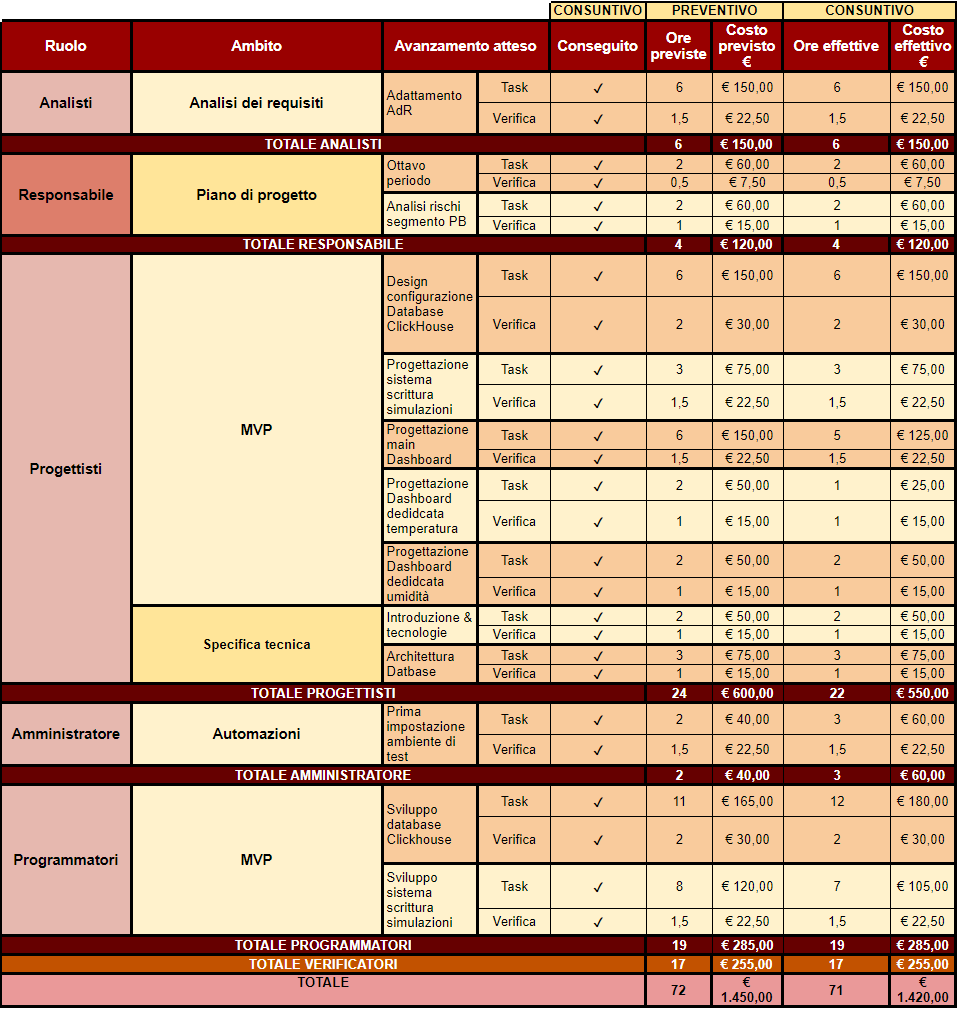
\includegraphics[height=1.1\textwidth]{../Images/periodo8.PNG}
    \caption{Ottavo periodo}
    \label{fig:Ottavo_periodo}
\end{figure}

Al termine dell'ottavo periodo, l'ammontare totale del costo del progetto è \textbf{6012,50\euro} e sono state completate il \textbf{100\%} delle \textit{attività}\textsubscript{\textit{G}} attese.
Il preventivo a finire rimane invariato a \textbf{12425,00\euro} e non risulta necessaria una ripianificazione delle \textit{attività}\textsubscript{\textit{G}} future.
\href{https://github.com/orgs/ByteOps-swe/projects/3/views/1?sortedBy%5Bdirection%5D=asc&sortedBy%5BcolumnId%5D=64182560}{Vai al Diagramma di Gantt.}

\begin{figure}[H]
    \centering
    \begin{minipage}[b]{0.70\textwidth}
        \centering
        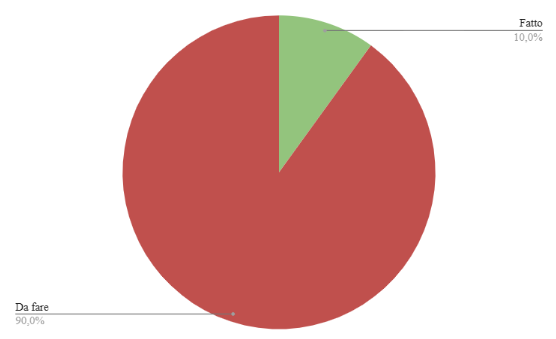
\includegraphics[width=0.7\textwidth]{../Images/avanzamento8Periodo.png}
        \caption{Avanzamento dei lavori RTB - Ottavo periodo}
        \label{fig:Avanzamento_RTB_8}
    \end{minipage}
\end{figure}

\paragraph{Preventivo orario}

\begin{figure}[H] 
    \centering
    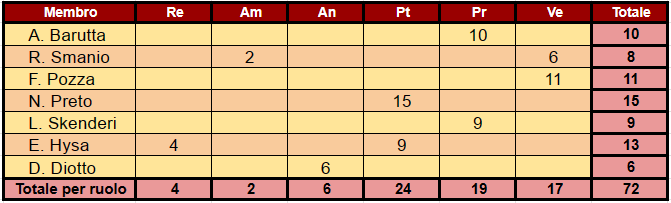
\includegraphics[width=0.9\textwidth]{../Images/preventivoOrario8Periodo.png}
    \caption{Preventivo orario per membro - Ottavo periodo}
    \label{fig:Preventivo_orario_8}
\end{figure}

\begin{figure}[H]
    \centering
    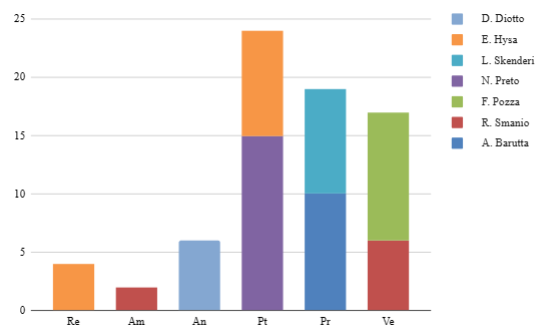
\includegraphics[width=0.6\textwidth]{../Images/preventivoDivisioneRuoli8Periodo.png}
    \caption{Istogramma preventivo della ripartizione oraria dei ruoli - Ottavo periodo}
    \label{fig:Preventivo_ripartizione_oraria_8}
\end{figure}

\paragraph{Consuntivo orario}

\begin{figure}[H]
    \centering
    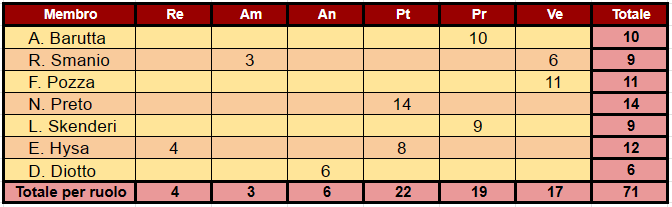
\includegraphics[width=0.9\textwidth]{../Images/consuntivoOrario8Periodo.png}
    \caption{Consuntivo orario per membro - Ottavo periodo}
    \label{fig:Constuntivo_orario_8}
\end{figure}

\begin{figure}[H]
    \centering
    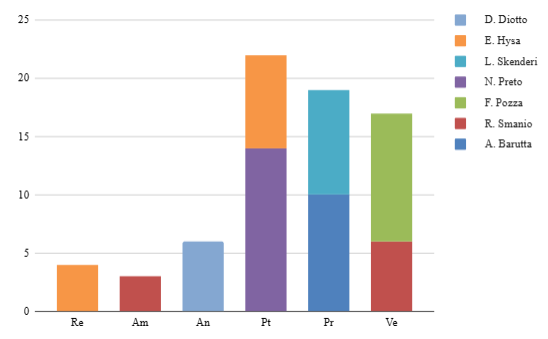
\includegraphics[width=0.6\textwidth]{../Images/consuntivoDivisioneRuoli8Periodo.png}
    \caption{Istogramma consuntivo della ripartizione oraria dei ruoli - Ottavo periodo}
    \label{fig:Consuntivo_ripartizione_oraria_8}
\end{figure}


%---------------------NONO PERIODO---------------------------------------

\subsubsection{Nono periodo  23/02/2024 - 01/03/2024}

\paragraph{Considerazioni}

\paragraph{Gestione dei rischi} \todo{completa}

\begin{itemize}
    \item \textbf{Rischi attesi e verificati:}
    \begin{itemize}
        \item \textbf{ID} - \textcolor{red}{rischio 1 (\textit{riferimento})} 
        \item \textbf{ID} - \textcolor{red}{rischio 2 (\textit{riferimento})} 
    \end{itemize}
\item \textbf{Rischi attesi ma non verificati:}
    \begin{itemize}
        \item \textbf{ID} - \textcolor{red}{rischio 1 (\textit{riferimento})}
        \item \textbf{ID} - \textcolor{red}{rischio 2 (\textit{riferimento})}
    \end{itemize} 
\item \textbf{Rischi non attesi ma verificati:}
    \begin{itemize}
        \item \textbf{ID} - \textcolor{red}{rischio 1 (\textit{riferimento})}
    \end{itemize}
\end{itemize}


\paragraph{Definizione ruoli}
Per le \textit{attività}\textsubscript{\textit{G}} registrate nei costi, sono stati assegnati i seguenti ruoli: 

\begin{table}[H]
    \centering
    \begin{tabular}{|L{4cm}|L{2cm}|}
        \hline
        \textbf{Ruolo} & \textbf{Persona} \\
        \hline
        \hline
        Responsabile (Re)   & L. Skenderi \\
        \hline
        Amministratore (Am) & F. Pozza \\
        \hline
        Analisti (An)       & L. Skenderi \\
        \hline
        Verificatore (Ve)   & E. Hysa \\
                            & N. Preto \\
                            & A. Barutta \\
                            & L.Skenderi \\   
        \hline
        Programmatori (Pr)  & R. Smanio \\
                            & D. Diotto \\
        \hline
        Progettista (Pt)    & A. Barutta \\
                            & F. Pozza \\
        \hline
    \end{tabular}
    \caption{Tabella dei ruoli assegnati - Nono periodo}
    \label{tab:Ruoli_persone_9}
\end{table}

\paragraph{Pianificazione attività divise per ruoli con consuntivo e preventivo orario e dei costi}

\vspace{0.4cm}

\begin{figure}[H]
    \centering
    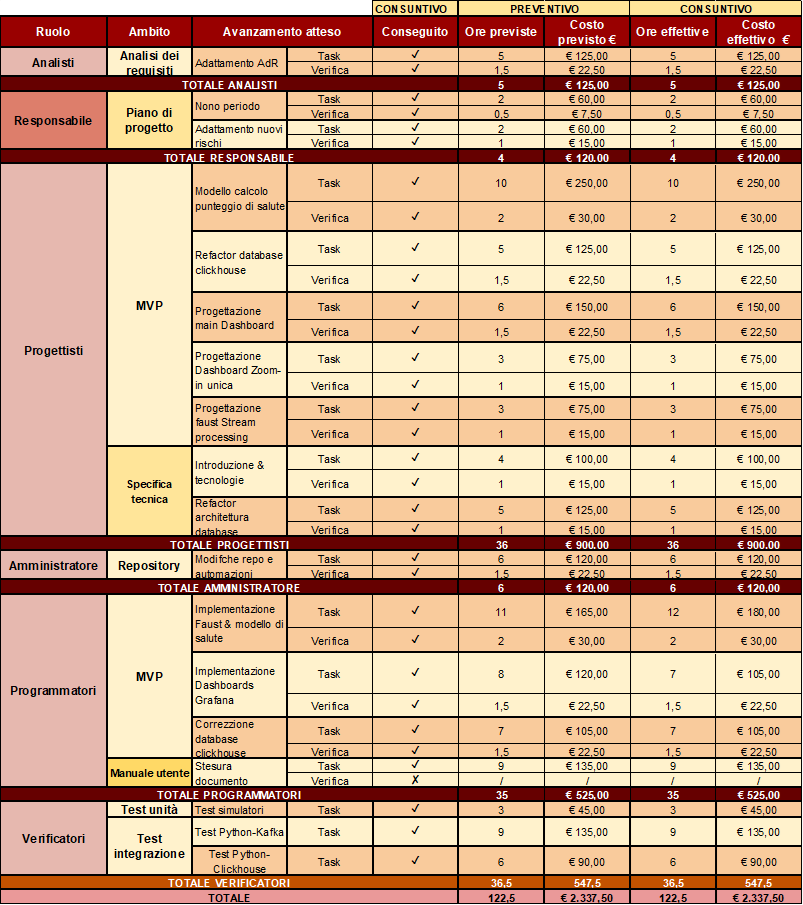
\includegraphics[height=1.1\textwidth]{../Images/periodo9.PNG}
    \caption{Nono periodo}
    \label{fig:Nono_periodo}
\end{figure}

Al termine del nono periodo, l'ammontare totale del costo del progetto è \textcolor{red}{\textbf{XXX \euro}}\todo{inserisci} e sono state completate il \textbf{100\%} delle \textit{attività}\textsubscript{\textit{G}} attese.
Il preventivo a finire rimane invariato a \textbf{12425,00\euro} e non risulta necessaria una ripianificazione delle \textit{attività}\textsubscript{\textit{G}} future.
\href{https://github.com/orgs/ByteOps-swe/projects/3/views/1?sortedBy%5Bdirection%5D=asc&sortedBy%5BcolumnId%5D=64182560}{Vai al Diagramma di Gantt.}

\begin{figure}[H]
    \centering
    \begin{minipage}[b]{0.70\textwidth}
        \centering
        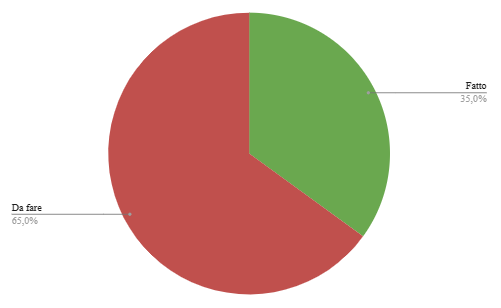
\includegraphics[width=0.7\textwidth]{../Images/avanzamento9Periodo.png}
        \caption{Avanzamento dei lavori RTB - Nono periodo}
        \label{fig:Avanzamento_RTB_9}
    \end{minipage}
\end{figure}

\paragraph{Preventivo orario}

\begin{figure}[H] 
    \centering
    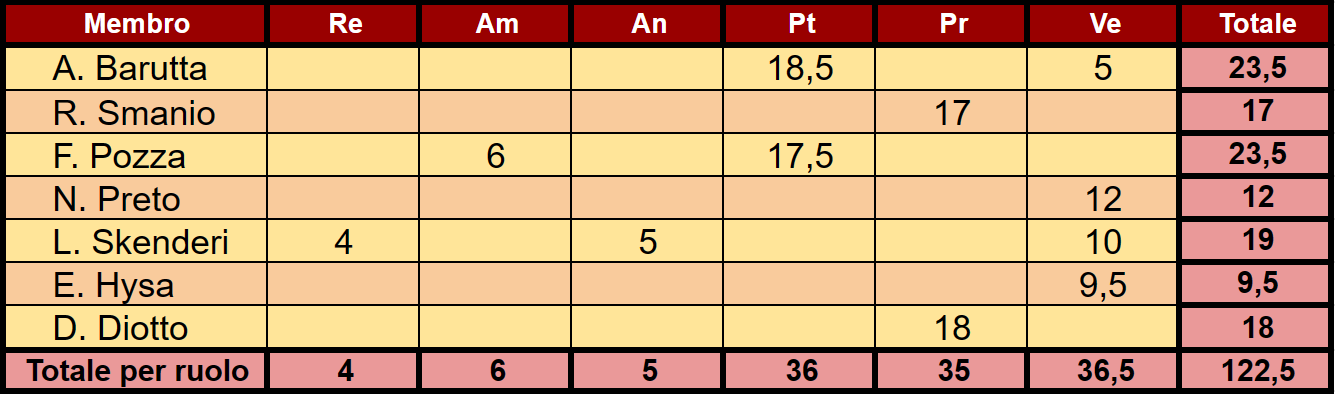
\includegraphics[width=0.9\textwidth]{../Images/preventivoOrario9Periodo.png}
    \caption{Preventivo orario per membro - Nono periodo}
    \label{fig:Preventivo_orario_9}
\end{figure}

\begin{figure}[H]
    \centering
    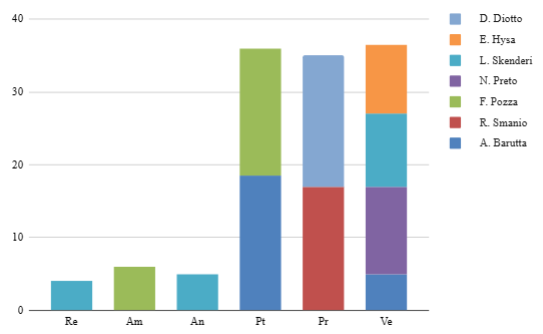
\includegraphics[width=0.6\textwidth]{../Images/preventivoDivisioneRuoli9Periodo.png}
    \caption{Istogramma preventivo della ripartizione oraria dei ruoli - Nono periodo}
    \label{fig:Preventivo_ripartizione_oraria_9}
\end{figure}

\paragraph{Consuntivo orario}

\begin{figure}[H]
    \centering
    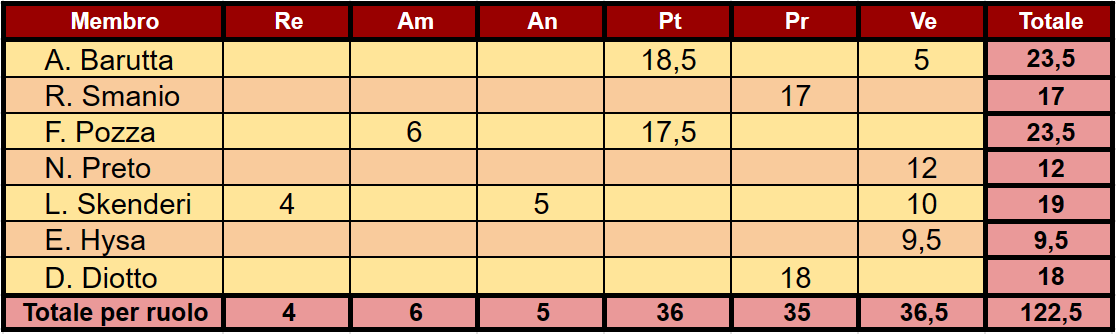
\includegraphics[width=0.9\textwidth]{../Images/consuntivoOrario9Periodo.png}
    \caption{Consuntivo orario per membro - Nono periodo}
    \label{fig:Constuntivo_orario_9}
\end{figure}

\begin{figure}[H]
    \centering
    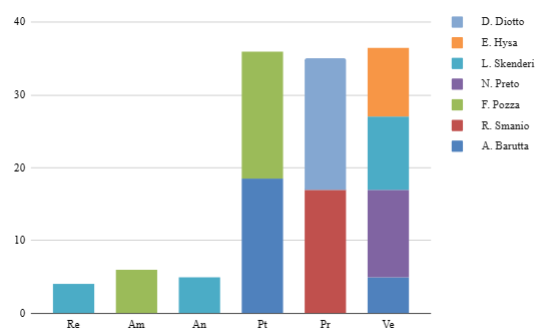
\includegraphics[width=0.6\textwidth]{../Images/consuntivoDivisioneRuoli9Periodo.png}
    \caption{Istogramma consuntivo della ripartizione oraria dei ruoli - Nono periodo}
    \label{fig:Consuntivo_ripartizione_oraria_9}
\end{figure}